%\documentclass{sig-alternate-05-2015}
\documentclass[10pt,conference]{IEEEtran}
%\documentclass{llncs}
\usepackage{makeidx}
\usepackage{tabularx,colortbl}
\usepackage[dvipsnames]{xcolor}
\usepackage{flushend}
\usepackage{cite}
\usepackage{amsmath}
\usepackage{amsthm}
\usepackage{amssymb}
\usepackage{epsfig}
\usepackage{stmaryrd}
\usepackage{url}
\usepackage{multirow}
\usepackage{latexsym}
\usepackage{graphics}
\usepackage{graphicx}
\usepackage{enumitem}
\usepackage{comment}
\usepackage{longtable}
\usepackage{supertabular}
\usepackage{times}
\usepackage{listings}
\usepackage{subfigure}
\usepackage{color}
\usepackage{balance}
\usepackage{xspace}
\usepackage[ruled, vlined, linesnumbered]{algorithm2e}
\usepackage[autostyle]{csquotes}



%\theoremstyle{Definition}
%\newtheorem{definition}{Definition}
%%%
%\theoremstyle{Theorem}
%\newtheorem{theorem}{Theorem}


%\newcommand{\definition}{\noindent \textbf{Definition} \citation{}}
%\newcommand{\theorem}{\noindent \textbf{Theorem} \citation{}}
%\newcommand{\lemma}{\noindent \textbf{Lemma} \citation{}}

%\newdef{lemma}{Lemma}
%\newdef{definition}{Definition}
%\newdef{theorem}{Theorem}
%\newdef{corollary}{Corollary}
%\newdef{note}{Note}
%\newdef{axiom}{Axiom}

\newtheorem{theorem}{Theorem}
\newtheorem{definition}{Definition}

\newcommand{\mkeyword}[1]{\mbox{\texttt{#1}}}
\DeclareMathOperator{\kuop}{uop}
\DeclareMathOperator{\kbop}{bop}
\DeclareMathOperator{\kite}{ite}
\DeclareMathOperator{\kpre}{pre}
\DeclareMathOperator{\dom}{dom}
\DeclareMathOperator{\ktrue}{true}
\DeclareMathOperator{\kfalse}{false}
\DeclareMathOperator{\kselect}{select}
\DeclareMathOperator{\ran}{range}
\newcommand{\lbb}{[\![}
\newcommand{\rbb}{]\!]}
\newcommand{\expr}{\phi}
\newcommand{\exprS}{\Phi}
\newcommand{\mike}[1]{\textcolor{red}{#1}}
\newcommand{\janet}[1]{\textcolor{blue}{#1}}
\newcommand{\darren}[1]{\textcolor{green}{#1}}
\newcommand{\danielle}[1]{\textcolor{orange}{#1}}

\sloppypar



\begin{document}

\definecolor{gold}{rgb}{0.90,.66,0}
\definecolor{dgreen}{rgb}{0,0.6,0}
\newcommand{\stateequiv}{\equiv_{s}}
\newcommand{\traceequiv}{\equiv_{\sigma}}
\newcommand{\ta}{\text{TA}}
\newcommand{\cta}{\text{TA$_{C}$}}
\newcommand{\tta}{\text{TA$_{T}$}}
\newcommand{\ucalg}{\texttt{\small{IVC\_UC}}}
\newcommand{\ucbfalg}{\texttt{\small{IVC\_UCBF}}}
\newcommand\doesnotentail{\mkern-2mu\not\mkern2mu\vdash}


\title{Using Inductive Validity Cores to Produce Minimal Cut Sets}
%


\author{\IEEEauthorblockN{Danielle Stewart\IEEEauthorrefmark{1}, Jing (Janet) Liu\IEEEauthorrefmark{2}, Michael W. Whalen\IEEEauthorrefmark{1}, Darren Cofer\IEEEauthorrefmark{2}, Mats Heimdahl\IEEEauthorrefmark{1}, Michael Peterson\IEEEauthorrefmark{3}}
\IEEEauthorblockA{\IEEEauthorrefmark{1}University of Minnesota\\Department of Computer
	Science and Engineering\\Email: \{dkstewar, whalen, heimdahl\}@umn.edu}
\IEEEauthorblockA{\IEEEauthorrefmark{2}Rockwell Collins\\
	Advanced Technology Center\\Email: \{Jing.Liu, Darren.Cofer\}@rockwellcollins.com}
\IEEEauthorblockA{\IEEEauthorrefmark{3}Rockwell Collins\\
	Commercial Systems Flight Controls Safety Engineering\\Email: Michael.Peterson@rockwellcollins.com}}


\maketitle

\begin{abstract}
Risk and fault analysis are important activities that help to ensure that critical systems operate in an expected way. As critical systems become more dependent on software components, analysis regarding fault propagation through these software components becomes more important. The methods used to perform these analyses require understandability from the side of the analyst, scalability in terms of system size, and mathematical correctness in order to provide sufficient proof that a system is safe. Determination of the events that can cause failures to propagate through a system as well as the affects of these propagations can be a time consuming and error prone process. In this paper, we describe a technique for determining these events with the use of a model checker and producing compositionally derived artifacts that encode pertinant system safety information. We describe the technique of generating these safety artifacts, prove that our approach is sound, and describe its implementation in the Osate tool suite for AADL. We then present experiments in which we benchmark our approach in terms of scalability and the artifacts produced.
\end{abstract}

\section{Introduction}

System safety analysis techniques are well established and are a required activity in the development of commercial aircraft and safety-critical ground systems. However, these techniques are based on informal system descriptions that are separate from the actual system design artifacts, and are highly dependent on the skill and intuition of a safety analyst. The lack of precise models of the system architecture and its failure modes often forces safety analysts to devote significant effort to gathering architectural details about the system behavior from multiple sources and embedding this information in safety artifacts, such as fault trees.

While model-based development (MBD) methods are widely used in the aerospace industry, they are generally disconnected from the safety analysis process itself. Formal model-based systems engineering (MBSE) methods and tools~\cite{QFCS15:backes,hilt2013,NFM2012:CoGaMiWhLaLu,DBLP:journals/scp/CimattiT15,Pajic2012,DBLP:conf/adaEurope/SokolskyLC09} now permit system-level requirements to be specified and analyzed early in the development process. These tools can also be used to perform safety analysis based on the system architecture and initial functional decomposition. Design models from which aircraft systems are developed can be integrated into the safety analysis process to help guarantee accurate and consistent results. This integration is especially important as the amount of safety-critical hardware and software in domains such as aerospace, automotive, and medical devices has dramatically increased due to desire for greater autonomy, capability, and connectedness.

Architecture description languages, such as SysML~\cite{SysML} and the Architecture Analysis and Design Language (AADL)~\cite{AADL} are appropriate for capturing system safety information.  There are several tools that currently support reasoning about faults in architecture description languages, such as the AADL error annex~\cite{Larson:2013:IAE:2527269.2527271} and HiP-HOPS for EAST-ADL~\cite{CHEN201391}.  However, these approaches primarily use {\em qualitative} reasoning, in which faults are enumerated and their propagations through system components must be explicitly described.  Given many possible faults, these propagation relationships become complex and it is also difficult to describe temporal properties of faults that evolve over time (e.g., leaky valve or slow divergence of sensor values).

In earlier work, University of Minnesota and Rockwell Collins developed and demonstrated an approach to model-based safety analysis (MBSA) \cite {Joshi05:Dasc,Joshi05:SafeComp,NasaRep:MBSA-Aug05} using the Simulink notation \cite{MathWorks}.  In this approach, a behavioral model of (sometimes simplified) system dynamics was used to reason about the effect of faults.  We believe that this approach allows a natural and implicit notion of fault propagation through the changes in pressure, mode, etc. that describe the system's behavior.  Unlike qualitative approaches, this approach allows uniform reasoning about system functionality and failure behavior, and can describe complex temporal fault behaviors.  On the other hand, Simulink is not an architecture description language, and several system engineering aspects, such as hardware devices and non-functional aspects cannot be easily captured in models.

\iffalse
Over the last five years, several research groups have focused on formal reasoning at the system architecture level, resulting in MBSE tools that incorporate assume-guarantee compositional reasoning techniques~\cite{Trento and Rockwell and UMN}.  These tools allow behavioral reasoning about complex system models, but with substantially greater scalability than previous approaches.
\fi

This paper describes our initial work towards a behavioral approach to MBSA using AADL.  Using assume-guarantee compositional reasoning techniques, we hope to support system safety objectives of ARP4754A and ARP4761.  To make these capabilities accessible to practicing safety engineers, it is necessary to extend modeling notations to better describe failure conditions, interactions, and mitigations, and provide improvements to compositional reasoning approaches focused on the specific needs of system safety analysis.  These extensions involve creating models of fault effects and weaving them into the analysis process.  To a large extent, our work has been an adaptation of the work of Joshi et. al to the AADL modeling language.

To evaluate the effectiveness and practicality of our approach, we developed an architectural model of the Wheel Braking System model in SAE AIR6110.  Starting from a reference AADL model constructed by the SEI instrumented with qualitative safety analysis information~\cite{SEI:AADL}, we added behavioral contracts to the model.  In so doing, we determine that there are errors related to (manually constructed) propagations across components, and also an architecture that contains single points of failure.  We use our analyses to find and fix these errors.

The rest of the paper is organized as follows...





\section{Model-Based Safety Analysis}

\mike{Audience should already know about model-based safety analysis.  We want to discuss two ``strands'' of MBSA, one with explicit fault propagation of faults rather than system dynamics, and another based on faults propagating through their effects on dynamics}.

A model-based approach for safety analysis was first proposed by Joshi et. al in \cite{Joshi05:Dasc, Joshi05:SafeComp, Joshi07:Hase}.  In this approach, a safety analysis system model (SASM) is the central artifact in the safety analysis process, and traditional safety analysis artifacts, such as fault trees, are automatically generated by tools that analyze the SASM. Figure~\ref{fig:sasm} provides an overview of this process applied to the wheel braking system example.

The contents and structure of the SASM differ significantly across different conceptions of MBSA.  We can draw broad outlines between two different approaches: one in which {\em faults} are propagated between components explicitly and the analysis proceeds by determining the likelihood of faults to system boundaries, and another in which faults propagate by changing the system dynamics, which may cause the system behavior to visibly change.  We call the first style the {\em explicit fault propagation} and the second style {\em implicit fault propagation} or {\em behavioral} propagation.

We contrast these two styles below...

\mike{Regurgitate content from "Model-Based Safety Analysis with smartIflow"}
\danielle{I added the citation from this paper to the bib file: cite\{info17:HaLuHo\} in case we want to use it.} \cite{info17:HaLuHo}.

\mike{Some contrasting points: richness of dynamics.  Most tools use formalisms that can only represent discrete quantities; we can do real-valued or large-domain integer dynamics}


\mike{Also we are explicitly integrated with an architecture language}


\subsection{Explicit Fault Propagation Approaches}



\mike{What is being done in AltaRica, HiPHOPS, AADL Error Annex...more here about primacy of faults as the mechanism of propagation between components.  Steal from proposal.}
\danielle{I added a few things from the proposal regarding fault propagation between components. There is a note below where that begins. I am not sure which papers you are referring to here so I can't really dig into those...}

The explicit propagation approach focuses on faults rather than constructing a model of system dynamics.

We illustrate this approach with the AADL error model annex~\cite{SAEAS} that can be used to describe system behaviors in the presence of faults. This annex has facilities for defining error types which can be used to describe error events that indicate errors in the system. The behavior of system components in the presence of errors is determined by state machines that are attached to system components; these state machines can determine error propagations and error composition for systems created from various subcomponents.

Error types in this framework are a set of enumeration values such as NoData, BadData, LateDelivery, EarlyDelivery, TimingError, and NoService. These errors can be arranged in a hierarchy. For example, LateDelivery and EarlyDelivery are subtypes of TimingError. The errors do not have any information (other than their type) associated with them. AADL includes information on the bindings of logical components (processes, threads, systems) and their communication mechanisms onto physical resources (memories, processors, busses), and the error annex uses this information to describe how physical failures can manifest in logical components.

\begin{figure}
  \centering
 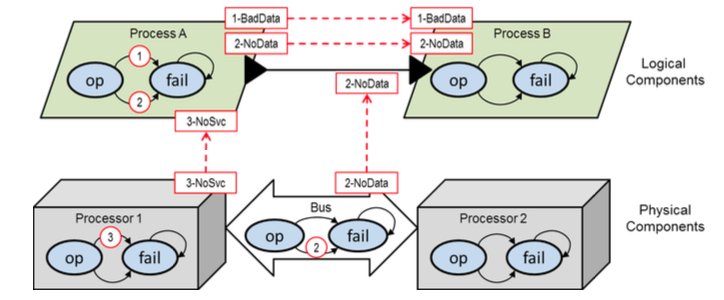
\includegraphics[width=0.75\textwidth]{images/error_annex.png}
  \vspace{-0.1in}
  \caption{Example of Error Model Information and Propagation}
  \label{fig:error_annex}
\end{figure}

An example is shown in Figure~\ref{fig:error_annex} \mike{Where is this figure?!?} \danielle{It was in the MBSA section. I have moved it here and if needed will reference from there}. Errors are described by the red rectangles labeled with error types: 1-BadData, 2-NoData, 3-NoSvc. Error events that can cause a component to fail are labeled with the corresponding error number. The error behavior of components is described by their state machines. Note that while all state machines in Figure 2 have two states, they can be much more complex. The red dashed arrows indicate propagations describing how failures in one component can cause other components to fail. For example, failures in the physical layer propagate to failures in the associated logical components.

Although the error model annex is very capable, it is not closely tied to the behavioral model of components or their requirements. For example, in the wheel braking system (WBS) example \cite{AIR6110}, it is possible that hydraulic system valves can fail open or fail closed. In fail closed, downstream components receive no flow and upstream pipes may become highly pressurized as a natural consequence of the failure. Physical models of these behavioral relationships often exist that can propagate failures in terms of the behavioral relationships between components. However, with the AADL error model annex, the propagations must be (re)specified and defined for each component. The user must therefore model the system twice, specifying propagations in the models of the physical phenomena, and again using enumerations and propagation rules in state machines in the error model annex. This re-specification can lead to inconsistencies between physical models and error annex models. In addition, the physical relationships between failures can be complex and may not be describable using enumeration values, leading to additional inconsistencies between the behavior of the physical phenomenon and the behavior of the error model.

\danielle{Added from proposal. I believe this describes what you mentioned above, Mike.}
This research attempts to bridge the descriptions of errors in the error model annex with behavioral descriptions of components. We start from the error model notions of error types and state machines that describe transitions from nominal to error states. However, we then tie these nominal and error states to behavioral models of the components in question that describe how the faults manifest themselves in terms of the signals or quantities produced by the components. Now the behavioral models can provide implicit propagation of the faulty behaviors and the natural consequences of failures on component behavior will be manifested in the propagation of other component faults through the behavioral model.

To accomplish this, we use AADL and the error model annex to describe faults and to use the AGREE contract specification language to describe behavioral models. This will require extensions to AGREE to define fault models that describe how different faults manifest themselves in changes to output signals. It will also require changes to the error annex. The conditions under which faults occur will become richer such that they describe not just propagation of enumerations from other components, but also valuations of input signals. For example, very high pressure in a pipe in the WBS model may lead to a \textit{pipe burst} failure. 


\subsection{Implicit Fault Propagation Approaches (Behavioral MBSA)}

\mike{Unfortunately, this is what is done, and done well in xSAP; they have a CAV paper on it; need to account for this}.
\danielle{I have been trying to find this paper... not sure what it is. I will move on for now and perhaps you have the paper title so that I can add a citation and some accounting for their research.}

The analysis starts from a {\em nominal} model of the system that describes the system behavior when no faults are present.  To perform safety analysis, we then also formalize the fault model. The fault model, in addition to common failure modes like \emph{non-deterministic}, \emph{inverted}, \emph{stuck\_at} etc, could encode information
regarding fault propagation, simultaneous dependent faults and fault hierarchies, etc.
After specifying the fault model and composing it with the original system model, the safety analysis involves verifying whether the safety requirements hold in presence of the faults defined in the fault model.


In this work, a behavior fault modeling language was constructed as an extension to the Lustre language \cite{Halbwachs91:IEEE}. Lustre is the kernel language of the popular model-based development tool SCADE \cite{SCADE}. In this approach, a safety engineer can model different kinds of fault behavior: e.g., stuck-at, ramp-up, ramp-down, and nondeterministic, and then {\em weave} these fault models into the nominal model. The language for describing faults is extensible, allowing engineers to define a catalog of faults appropriate for their domain. In addition, the weaving process allows error propagation between unconnected components within a system model \cite{Joshi07:Hase}. This allows consideration of physical aspects (e.g., proximity of components, shared resources such as power) that may not be present in a logical system model but can lead to dependent failures. In addition, it allows propagation of faults in the reverse direction of the model data flow. This can occur when physical components have coupling such as back-pressure in fluid systems or power surges in the opposite direction of communication through connected components. Finally, it is possible to create fault mediations to describe the output in the presence of multiple simultaneous faults.



%In previous work, component-level modeling tools such as Simulink \cite{MathWorks} and SCADE \cite{SCADE} were extended. In this work, we adapt this process to target system architecture models \cite{AADL, SysML} for safety analysis.

%\subsection{Safety Analysis Approach}
\begin{figure}
  \centering
 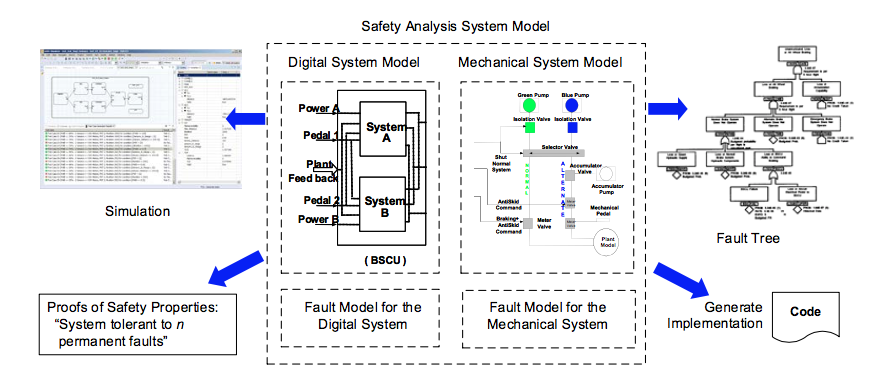
\includegraphics[width=1\textwidth]{images/SASM.png}
  \vspace{-0.1in}
  \caption{Safety Analysis System Model}
  \label{fig:sasm}
\end{figure}

A safety analysis system model can be used for a variety of simulations and analyses as shown in Figure~\ref{fig:sasm} \mike{include figure?} \danielle{Do you mean a figure like this one? If not, I can change it (I got it from the proposal) If so, perhaps Darren has a nonblurry copy of the figure? I can't get this one to be more clear...}. Modeling allows trivial exploration of \textit{what-if} scenarios involving combinations of faults through simulations. For more rigorous analyses, static analysis tools, such as model checkers and theorem provers, can be used to automatically prove (or disprove) whether the system meets specific safety requirements.
The primary approach used for analysis in previous work was model checking. After creating the system model, a model checker was used to verify that safety properties hold on the nominal system, an idealized model of the digital controller and the mechanical system containing no faults. Once the nominal model is shown to satisfy the safety property, the behavior of the fault-extended model can be examined. In the approach described by Joshi et al. in \cite{Joshi05:Dasc, Joshi05:SafeComp, Joshi07:Hase}, this analysis was performed by determining whether the property held for a given fault threshold: the maximum number of component faults to which the system is expected to be resilient.

This fault threshold is, in some sense, an approximation of the likelihood of component faults. It maps from the probabilistic \textit{real world} potential for component failure into a non-probabilistic verification problem. Recent work \cite{CAV2015:BoCiGrMa} uses a more sophisticated approach involving minimum cut sets to describe the set of potential component failures that must be considered. Both approaches provide separation between the probabilistic aspects of the real world and the computational demands of formal analysis. This approach currently scales far better than direct use of probabilistic model checking tools such as PRISM \cite{CAV2011:KwNoPa}, and will likely continue to do so in the future.

\iffalse
\subsection{Compositional Verification of System Architectures}

As part of the NASA Compositional Verification of Flight Critical Systems (CVFCS) project and the DARPA META and High Assurance Cyber Military Systems (HACMS) projects, we have constructed sophisticated compositional verification tools for reasoning about complex systems architectures. These tools \cite{NFM2012:CoGaMiWhLaLu} allow scaling of formal verification through splitting the analysis of a complex system architecture into a collection of verification tasks that correspond to the structure of the architecture. By decomposing the verification effort into proofs about each subsystem within the architecture, the analysis has been scaled to very large system designs \cite{QFCS15:backes}. In the case of the software for a complex medical drug infusion pump, a monolithic analysis of the design does not terminate in 24 hours, while the compositional approach completes in just over five minutes.
<<<<<<< HEAD
The approach naturally supports an architecture-based notion of requirements refinement based on assume-guarantee contracts. The properties of components necessary to prove a system-level property, including any assumptions about the component environment, in effect define the requirements for those components. The approach allows reuse of the verification that must already be performed on safety-critical software components and enables distributed development by establishing the formal contracts for components that are used to assemble a system architecture. If we are able to establish a system property using only the contracts of its components, we have the means for performing virtual integration of the components. We can use the contract of each component as a specification for suppliers and have a great deal of confidence that if all the suppliers meet their specifications, the integrated system will work properly.
We have implemented this assume-guarantee mechanism for compositional verification as an extension of the AADL language derived from the safety property subset of the property specification language (PSL) \cite{IEEE:PSL}. The Assume-Guarantee Reasoning Environment (AGREE) is our tool for compositional verification of these contracts. Under the CVFCS project, we are currently adding automated bi-directional translation between AGREE contracts and implementation-level properties in languages such as C and Simulink. Initially, we will support translation into MATLAB properties for analysis using the Simulink Design Verifier and C assertions for analysis using source code model checkers (such as CMBC) or test- based verification. Since contracts are abstractions of component implementations, they provide a much more efficient way of representing heterogeneous components in the system model than translating the component models themselves.
=======

The approach naturally supports an architecture-based notion of requirements refinement based on assume-guarantee contracts. The properties of components necessary to prove a system-level property, including any assumptions about the component environment, in effect define the requirements for those components. The approach allows reuse of the verification that must already be performed on safety-critical software components and enables distributed development by establishing the formal contracts for components that are used to assemble a system architecture. If we are able to establish a system property using only the contracts of its components, we have the means for performing virtual integration of the components. We can use the contract of each component as a specification for suppliers and have a great deal of confidence that if all the suppliers meet their specifications, the integrated system will work properly.

We have implemented this assume-guarantee mechanism for compositional verification as an extension of the AADL language derived from the safety property subset of the property specification language (PSL) \cite{IEEE:PSL}. The Assume-Guarantee Reasoning Environment (AGREE) is our tool for compositional verification of these contracts. Under the CVFCS project, we are currently adding automated bi-directional translation between AGREE contracts and implementation-level properties in languages such as C and Simulink. Initially, we will support translation into MATLAB properties for analysis using the Simulink Design Verifier and C assertions for analysis using source code model checkers (such as CMBC) or test- based verification. Since contracts are abstractions of component implementations, they provide a much more efficient way of representing heterogeneous components in the system model than translating the component models themselves.

>>>>>>> 705062d4005b55c503d3e85e228be8e236a1ac1e

\fi



\section{Methodology}

The details of implementation and formalisms. 

\subsection{Preliminaries}

\subsubsection{Inductive Validity Cores}
Given a complex model, it is often useful to extract traceability information related to the proof, in other words, which portions of the model were necessary to construct the proof. To this end, an algorithm was developed that efficiently computes the \textit{inductive validity cores} (IVC) within a model necessary for the proofs of safety properties for sequential systems \cite{DBLP:journals/corr/GhassabaniGW16}. 

Given a state space $S$, a transition system $(I,T)$ consists of the initial state predicate $I : S \rightarrow \{0,1\}$ and a transition step predicate $T : S \times S \rightarrow \{0,1\}$. Reachability for $(I,T)$ is defined as the smallest predicate $R : S \rightarrow \{0,1\}$ which satisfies the following formulas:
\begin{center}
$\forall s. I(s) \Rightarrow R(s)$\\
$\forall s, s' .  R \land T(s,s') \Rightarrow R(s')$\\
\end{center}
A safety property $P : S \to \{0,1\}$ is a state predicate. A safety property $P$ holds on a transition system $(I,T)$ if it holds on all reachable states. More formally, $\forall s . R(s) \Rightarrow P(s)$. When this is the case, we write $(I,T) \vdash P$. Following Ghassabani, et. al. \cite{DBLP:journals/corr/GhassabaniGW16}, we formalize IVCs as follows.

\danielle{Find the correct way to add definitions, lemmas, etc. to this format.}\\
\textit{Definition 1: Inductive Validity Core:} Let $(I,T)$ be a transition system and let $P$ be a safety property with $(I,T) \vdash P$. Then $S \subseteq T$ is an \textit{inductive validity core} for $(I,T) \vdash P$ iff $(I,S) \vdash P$.  \\

\textit{Definition 1: Minimal Inductive Validity Core:} An inductive validity core $S$ for $(I,T) \vdash P$ is minimal iff $! \exists S' . S' \subset S \ni (I,S') \vdash P$. \\

\subsubsection{Fault Trees}
A fault tree is a directed acyclic graph (DAG) consisting of the node types \textit{events} and \textit{gates}. An event is an occurance within the system, typically the failure of a subsystem down to an individual component. Events can be grouped into \textit{basic events} (BEs), which occur independently, and \textit{intermediate events} which occur dependently and are caused by one or more other events. The event at the top of the tree, the \textit{top level event} (TLE), is the event being analyzed. This event models the failure of the system (or subsystem) under consideration. The gates represent how failures propagate through the system and how failures in subsystems can cause system wide failures. The following gates are often used in fault trees but this list is not comprehensive. \\
\textbf{AND} Output occurs if all of the input events occur.\\
\textbf{OR} Output occurs if any of the input events occur.\\

\danielle{There are obviously other forms of gates in fault trees (XOR, VOTING, INHIBIT, etc). I can define all of the gates that the Soteria model will be generating. That seems to make the most sense. Unless it really doesnät matter all that much. We can discuss.}\\

To formalize a fault tree (FT), we use $GateTypes = \{And, Or\}$. Following Ruijters, et. al. \cite{RuijtersSurvey}, we formalize FT as follows. 

\textit{Definition 3: Fault Tree:} A FT is a 4-tuple $F = \langle BE, G, T, I \rangle$ consisting of the following components. 
\begin{itemize}
\item BE is the set of basic events
\item G is the set of gates with $BE \cap G = \emptyset$. We write $E = BE \cup G$ for the set of elements.
\item $T: G \to GateTypes$ is a function that describes the type of each gate.
\item $I: G \to P(E)$ describes the inputs of each gate. We require that $I(G) \neq \emptyset$.
\end{itemize}

The graph formed by $\langle E, I \rangle$ is a directed acyclic graph with a unique root $TLE$ which is reachable from all nodes. 

\textit{Definition 4: Semantics of a Fault Tree:} The semantics of FT F is a function $\pi_F : P(BE) \times E \vdash \{0,1\}$ where $\pi_F(S, e)$ indicates whether $e$ fails given the set $S$ of failed BEs. It is defined as follows. 

\begin{itemize}
\item For $e \in BE$, $\pi_F(S,e) = e \in S$.
\item For $g \in G$ and $T(g) = And$, let\\ $\pi_F(S,g) = \land_{x \in I(g)} \pi_F(S, x)$
\item For $g \in G$ and $T(g) = Or$, let\\ $\pi_F(S,g) = \lor_{x \in I(g)} \pi_F(S, x)$ 
\end{itemize}

The interpretation of the TLE $t$ is written as $\pi_F(S,t) = \pi_F(S)$. If the failure of $S$ causes the TLE to occur, we write $\pi_F(S) = 1$. 

\subsection{Qualitative analysis}
Cut sets and minimal cut sets provide information about the vulnerabilities of a system in terms of its basic events. A \textit{cut set} is a set of components that together can cause a system to fail. A \textit{minimal cut set} is a cut set which contains the minimum number of basic events required in order to cause the TLE to occur. More formally, these are defined as follows. 

\textit{Definition 5: Cut Set:} $C \subseteq BE$ is a cut set of FT F if $\pi_F(C) = 1$. \\

\textit{Definition 6: Minimal Cut Set:} $C \subseteq BE$ is a MCS if $\pi_F(C) = 1 \land \forall C' \subset C. \pi_F(C') = 0$. In other words, a minimal cut set (MCS) is a cut set of which no subset is a cut set. 

\danielle{Can I say finding ALL min IVCs is the same as finding ALL MCSs? I have to make sure.}\\
Given the formalisms defined previously, we show that finding the minimal IVCs is equivalent to finding the MCS. \\

\textit{Theorem 1: Finding all minimal IVCs is equivalent to finding the set of all MCSs}:\\
\textit{Proof}: Let $T = \{f_1, f_2, ..., f_n\}$ be the set of model elements corresponding to faults for the components and let $P_{tle}$ be the top level event (TLE). By the definition for IVC, we know that $S \subseteq T$ is an IVC for $(I, T) \vdash P_{tle}$ iff $(I, S) \vdash P_{tle}$. 
In this case, we can quickly see that $\pi_F(S) = 1$, i.e. given the set $S \subseteq T$ of failed model elements, the top level event occurs. 
Since $S$ is minimal IVC, it follows that $\pi_F(M) = 0$ for any $M \subset S$ and hence the set of minimal IVCs is equivalent to the set of MCSs. 

\subsection{Quantitative analysis}
\danielle{I am going to really mess up notation for the moment and use the usual P for probability function. This messes up notation because I used it earlier to be a state predicate. I will change the predicate P later on since it makes the most sense to keep P as a probability function.}\\

Quantitative analysis methods derive numerical values for fault trees. One of these calculations that is of particular interest to the safety engineering community is the probability of the occurance of the top level event (TLE). The next section describes probability theory and provides a description of how we use these definitions in order to calculate the probability of the TLE. These definitions are based on the ones given in~\cite{RuijtersSurvey}.\\

\danielle{I will add the probability formalisms here later. For now, I just want to clarify my findings regarding the proof that Mike was talking about yesterday.}\\
Assume events occur independently. \\

Or gate: \\
Probability is defined as follows: \\
$P(A \lor B) = P(A) + P(B) - P(A \land B)$. \\
Assume that the probability of events A, B is quite small (this is called the Rare Event Approximation). Then the term $P(A \land B)$ will also be quite small and hence is an "error term". If we drop this term from the calculations, we end up with the approximated probability being: $P(A) + P(B) \geq P(A) + P(B) - P(A \land B)$. \\

And gate: \\
With the calculations of the and gate, this is where independence is really required. Using Bayes Rule, we have $P(A \land B) = P(B)P(A|B) = P(A)P(B|A)$ for conditionally dependent events and $P(A \land B) = P(B)P(A)$ for independent events. If we assume independence when the events are NOT independent, in the worst case scenario, we get something like $B$ is completely dependent on $A$. Therefore $P(B|A) = 1$ and $P(A \land B) = P(B) \geq P(B)P(A)$. Not a conservative estimation. In the case of dependence, joint probability values would be required (acommon cause analysis).  \\

\danielle{Any other kind of gate uses combinations of these rules. These are not proofs that I made, I just looked at the logic of the operations. I am not sure how much we want to include in the paper. I assume a description is necessary, but a proof? No, this isn't a proof... This is just following definitions down a short little jaunt in the woods.}








\section{Case Studies}

To demonstrate the effectiveness of this approach and compare to state of the art existing tools, we describe two case studies.

\subsection{Wheel Brake System}
The Wheel Brake System (WBS) described in AIR6110~\cite{AIR6110} is a well-known example that has been used as a case study for safety analysis, formal verification, and contract based design~\cite{DBLP:conf/cav/BozzanoCPJKPRT15, 10.1007/978-3-319-11936-6-7, CAV2015:BoCiGrMa, Joshi05:SafeComp}. The preliminary work for the safety annex used a simplified model of the WBS~\cite{Stewart17:IMBSA}. In order to demonstrate scalability of our tools and compare results with other studies, we constructed a functionally and structurally equivalent AADL version of one of the most complex WBS NuSMV/xSAP models (arch4wbs) described in~\cite{DBLP:conf/cav/BozzanoCPJKPRT15,mattareiThesis}. We refer readers to this publication for diagrams of the full arch4wbs model~\cite{DBLP:conf/cav/BozzanoCPJKPRT15}. A simplified diagram taken from ARP4761 is shown in Figure~\ref{fig:wbs_arp4761}. 

\begin{figure}[h]
\begin{center}
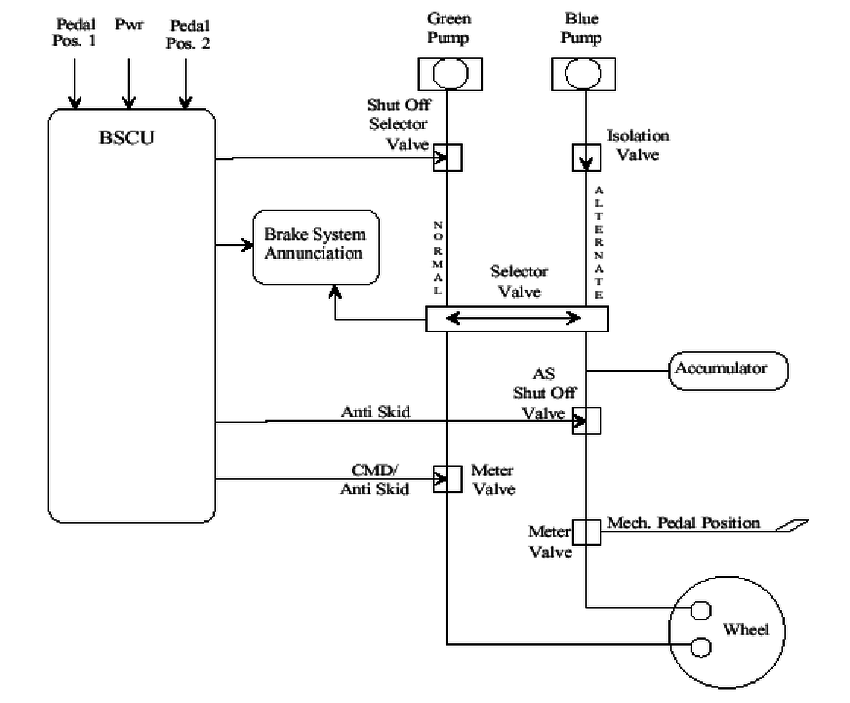
\includegraphics[width=8cm]{images/wbs_arp4761}
\caption{Simplified model of the WBS from ARP4761} \label{fig:wbs_arp4761}
\end{center}
\end{figure}

\subsubsection{WBS architecture description}
The WBS is composed of two main parts: the control system and the physical system. The control system electronically controls the physical system and contains a redundant Braking System Control Unit (BSCU) in case of failure. The physical system consists of the hydraulic circuits running from hydraulic pumps to wheel brakes. This is what provides braking force to each of the 8 wheels of the aircraft.

There are three operating modes in the WBS model. In \textit{normal} mode, the system uses the \textit{green} hydraulic circuit. The normal system is composed of the green hydraulic pump and one meter valve per each of the 8 wheels (shown as one wheel in Figure~\ref{fig:wbs_arp4761}). Each of the 8 meter valves are controlled through electronic commands coming from the BSCU. These signals provide brake commands as well as antiskid commands for each of the wheels. The braking command is determined through a sensor on the pilot pedal position. The antiskid command is calculated based on information regarding ground speed, wheel rolling status, and braking commands.

In \textit{alternate} mode, the system uses the \textit{blue} hydraulic circuit.  The wheels are all mechanically braked in pairs (one pair per landing gear). The alternate system is composed of the blue hydraulic pump, four meter valves, and four antiskid shutoff valves. The meter valves are mechanically commanded through the pilot pedal corresponding to each landing gear. If the system detects lack of pressure in the green circuit, the selector valve switches to the blue circuit. This can occur if there is a lack of pressure from the green hydraulic pump, if the green hydraulic pump circuit fails, or if pressure is cut off by a shutoff valve. If the BSCU channel becomes invalid, the shutoff valve is closed.

The last mode of operation of the WBS is the \textit{emergency} mode. This is supported by the blue circuit but operates if the blue hydraulic pump fails. The accumulator pump has a reserve of pressurized hydraulic fluid and will supply this to the blue circuit in emergency mode.

The model size and statistics are described in Table~\ref{fig:arch_table}. 

\begin{figure}[h]
\begin{center}
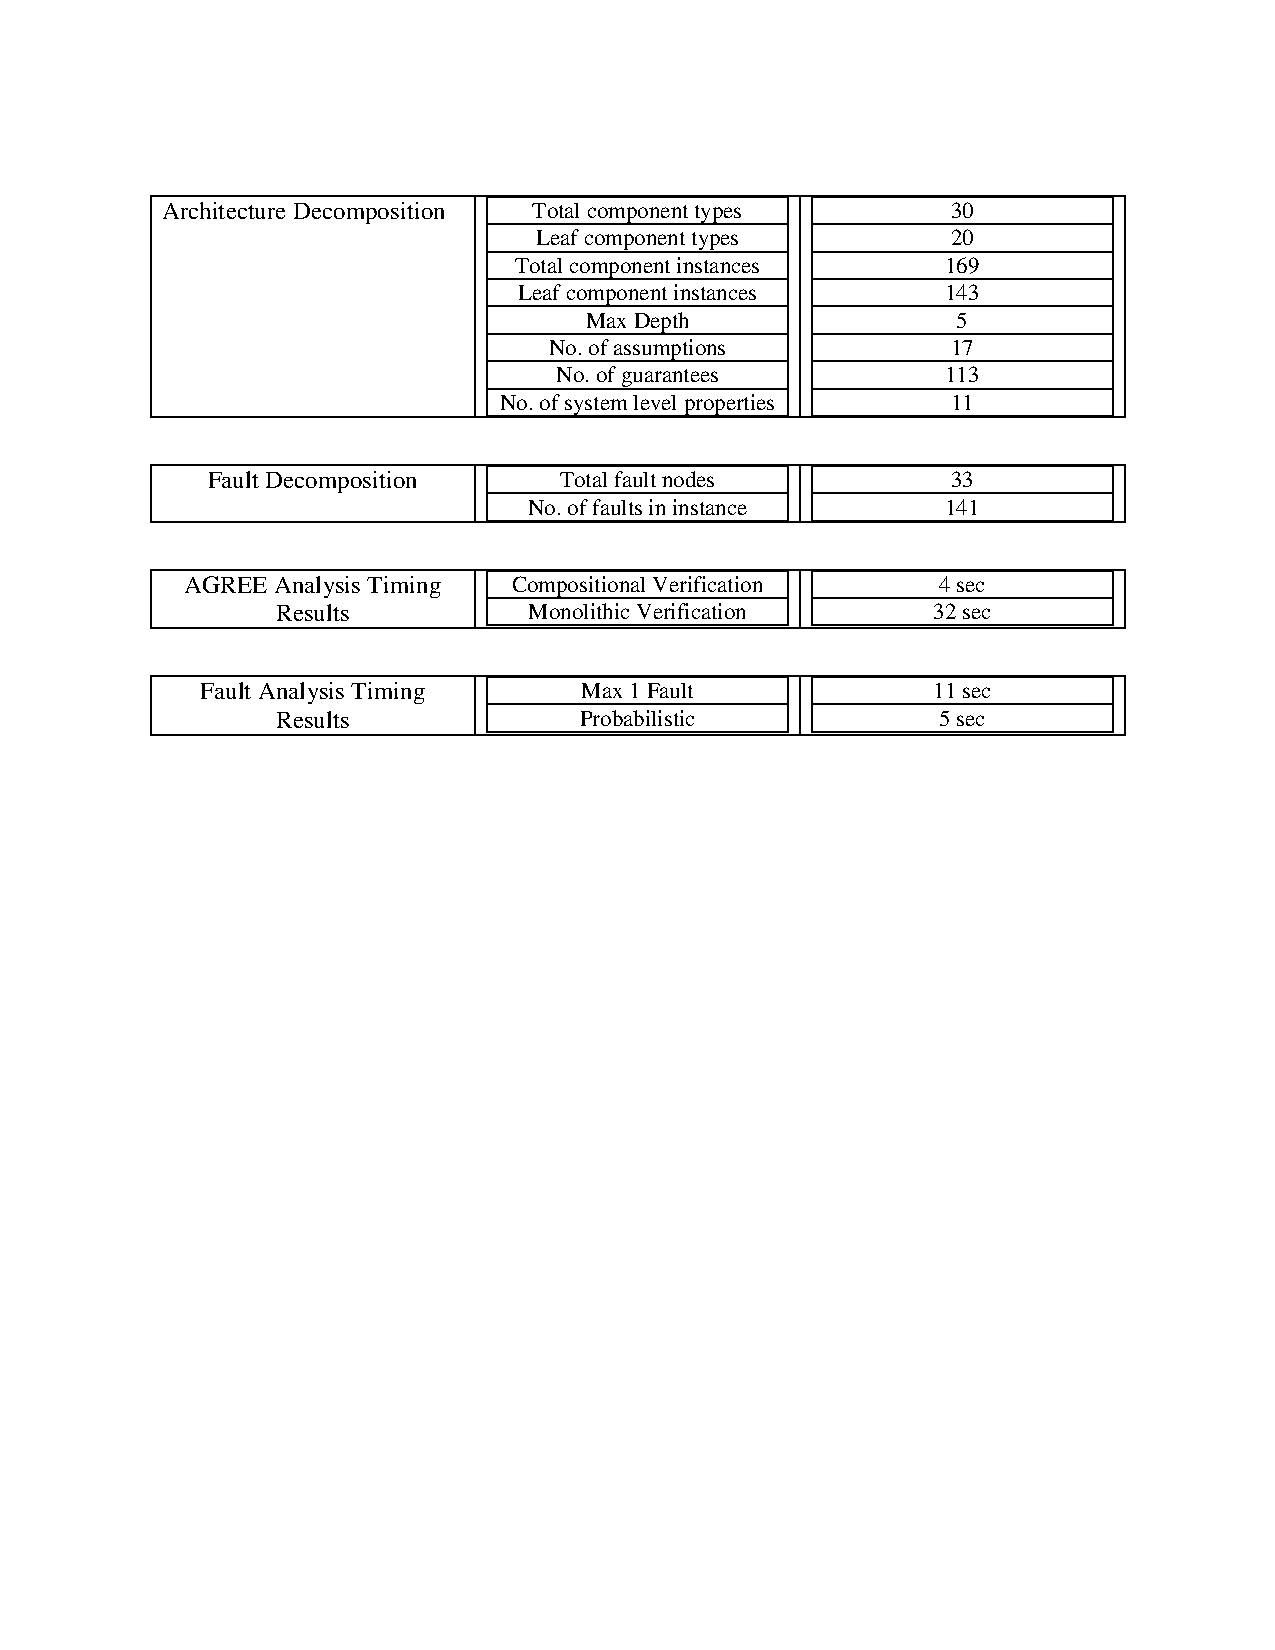
\includegraphics[width=8cm]{images/arch_table.png}
\caption{Model Statistics} \label{fig:arch_table}
\end{center}
\end{figure}

\subsubsection{System Safety Properties}
The AIR6110 document contains a set of safety requirements on the expected probability of an unwanted occurance of event, e.g. `'the loss of all wheel braking shall be extremely remote.'' The case study performed using xSAP/NuSMV~\cite{mattareiThesis, DBLP:conf/cav/BozzanoCPJKPRT15} focused on these safety requirements that are outlined in AIR6110. The detailed tech report of the xSAP/NuSMV model of the WBS can be found in~\cite{air6110TechReport}.

\textbf{S18-WBS-R-0321} \textit{Never loss of all wheel braking.}

\textbf{S18-WBS-R-0322-left} \textit{Never asymmetrical loss of wheel braking (left side).}

\textbf{S18-WBS-R-0322-right} \textit{Never asymmetrical loss of wheel braking (right side).}

\textbf{S18-WBS-0323} \textit{Never inadvertent braking with all wheels locked during takeoff roll before V1.}

\textbf{S18-WBS-R-0324} \textit{Never inadvertent braking of all wheels during takeoff roll after V1.}

\textbf{S18-WBS-R-0325-w1...8} \textit{Never inadvertent braking of one wheel without locking (wheels 1-8).} 

\textbf{Braking implies cmd w1...8} \textit{If system is braking, then pilot has commanded braking (wheels 1-8).} 

\textbf{Cmd implies braking w1...8} \textit{If pilot commands braking, then system is braking (wheels 1-8).} 

These requirements violations are the top level events (TLE) for the fault tree computations. 


\subsubsection{Qualitative analysis comparison}
\subsubsection{Quantitative analysis comparison}


\section{Related Work}
\label{sec:related_work}

%Address NFM review comments
In recent years, there has been an increase in the interest of Model Based Safety Analysis (MBSA)~\cite{Bozzano:2010:DSA:1951720}. 

Formal model based systems engineering (MBSE) methods and tools now permit system level requirements to be specified and analyzed early in the development process~\cite{QFCS15:backes,CIMATTI2015333, NFM2012:CoGaMiWhLaLu, hilt2013:MuWhRaHe, Pajic2012}. Design models from which aircraft systems are developed can be integrated into the safety analysis process to help guarantee accurate and consistent results. This integration is especially important as the amount of safety critical hardware and software has dramatically increased in safety critical domains such as aerospace, automotive, and medical fields~\cite{Stewart17:IMBSA}.

There are tools that currently support reasoning about faults in architecture description languages such as SysML and AADL. These tools include the AADL Error Model Annex, Version 2 (EMV2)~\cite{EMV2} and HiP-HOPS for EAST-ADL~\cite{CHEN201391}. These approaches primarily utilize \textit{qualitative} reasoning. Faults are enumerated and the propagations through system components are explicitly described. Given many possible faults, these propagation relationships increase in complexity and understandability. Interactions are easily overlooked by analysts and thus not explicitly described. This is also the case with tools like SAML that incorporate both \textit{qualitative} and \textit{quantitative} reasoning~\cite{Gudemann:2010:FQQ:1909626.1909813}. 

In earlier work, an approach to MBSA was demonstrated using the Simulink notation~\cite{Joshi05:SafeComp,Joshi05:Dasc,NasaRep:MBSA-Aug05, MathWorks} . In this approach, a behavioral model of system dynamics was used to reason about the effects of faults in the system. We believe this approach allows an implicit and natural notion of fault propagation through the system. Since Simulink is not an architecture description language, notions such as hardware devices and non-functional aspects cannot be captured in system models. Using this idea of \textit{quantitative} reasoning and implicit fault propagation, we wish to apply this to a more rich architecture language. 


Formal verification tools based on model checking have been used to automate the generation of safety artifacts and used in safety critical system certification~\cite{Bozzano:2011:SDP:1992983.1992988, symbAltaRica,10.1007/978-3-540-75596-8-13, DBLP:conf/tacas/BittnerBCCGGMMZ16, Bozzano:2010:DSA:1951720} . This approach has limitations in terms of scalability and readability of the fault trees generated. Work has been done to mitigate these limitations by the scalable generation of readable fault trees~\cite{10.1007/978-3-319-11936-6-7}. 

%Moved the following to case study
%The Wheel Brake System (WBS) described in ARP4761~\cite{SAE:ARP4761} has been used in the past as a case study for safety analysis, formal verification, and contract based design~\cite{DBLP:conf/cav/BozzanoCPJKPRT15, 10.1007/978-3-319-11936-6-7, CAV2015:BoCiGrMa, Stewart17:IMBSA, propBasedProofSys, Joshi05:SafeComp, NasaRep:MBSA-Aug05} The preliminary work for the safety annex used a simplified model of the WBS~\cite{Stewart17:IMBSA}. In order to show scalability and compare results with other studies, an AADL version of the WBS was designed based off of arch4wbs NuSMV model described in previous work~\cite{DBLP:conf/cav/BozzanoCPJKPRT15}. This model was chosen due to the number of subcomponents in the system and the complexity of behavior captured in the NuSMV model. 



\section{Conclusion}

We have developed an extension to the AADL language with tool support for formal analysis of system safety properties in the presence of faults. Faulty behavior is specified as an extension of the nominal model, allowing safety analysis and system implementation to be driven from a single common model. This new Safety Annex leverages the AADL structural model and nominal behavioral specification (using the AGREE annex) to propagate faulty component behaviors without the need to add separate propagation specifications to the model.   Next steps will include extensions to automate injection of Byzantine faults as well as automatic generation of fault trees.  For more details on the tool, models, and approach, see the technical report~\cite{SATechReport}.

\vspace{2 mm}
\noindent {\bf Acknowledgments.} This research was funded by NASA contract NNL16AB07T and the University of Minnesota College of Science and Engineering Graduate Fellowship.





%\vspace{-0.40cm}
\bibliographystyle{IEEEtran}

\bibliography{IEEEabrv,biblio}
%\vspace{-7.25cm}
% This ~ seems to fix an odd bibliography alignment issue


%\ifdefined\TECHREPORT
%\appendix
%
%\section{Appendix: Proof of Equivalence}
%\input{appendix}
%\fi

%\section{Appendix: GPCA CENTA Model}
%\label{appendix:gpcacenta}
%\begin{figure}[!ht]
%\begin{center}
%\includegraphics[scale=0.6]{images/sampled_pca.PNG} %[trim = 0 2 0 0, clip=true]{Comp}
%\caption{GPCA AGREE Properties modeled as a Timed Automata} \label{fig:samplepca}
%\end{center}
%\end{figure}

%\balancecolumns

\end{document} 